\cleardoublepage

\addcontentsline{toc}{chapter}{Anexos}

\titleformat{\chapter}{\fontsize{16pt}{5mm}\selectfont\bfseries}{\hspace{1cm}Anexo \thechapter}{1em}{}

\iffalse
\chapter{Especifica��o t�cnica Ardu�no}
\label{ArduinoAnexo}

\setboolean{@twoside}{false}
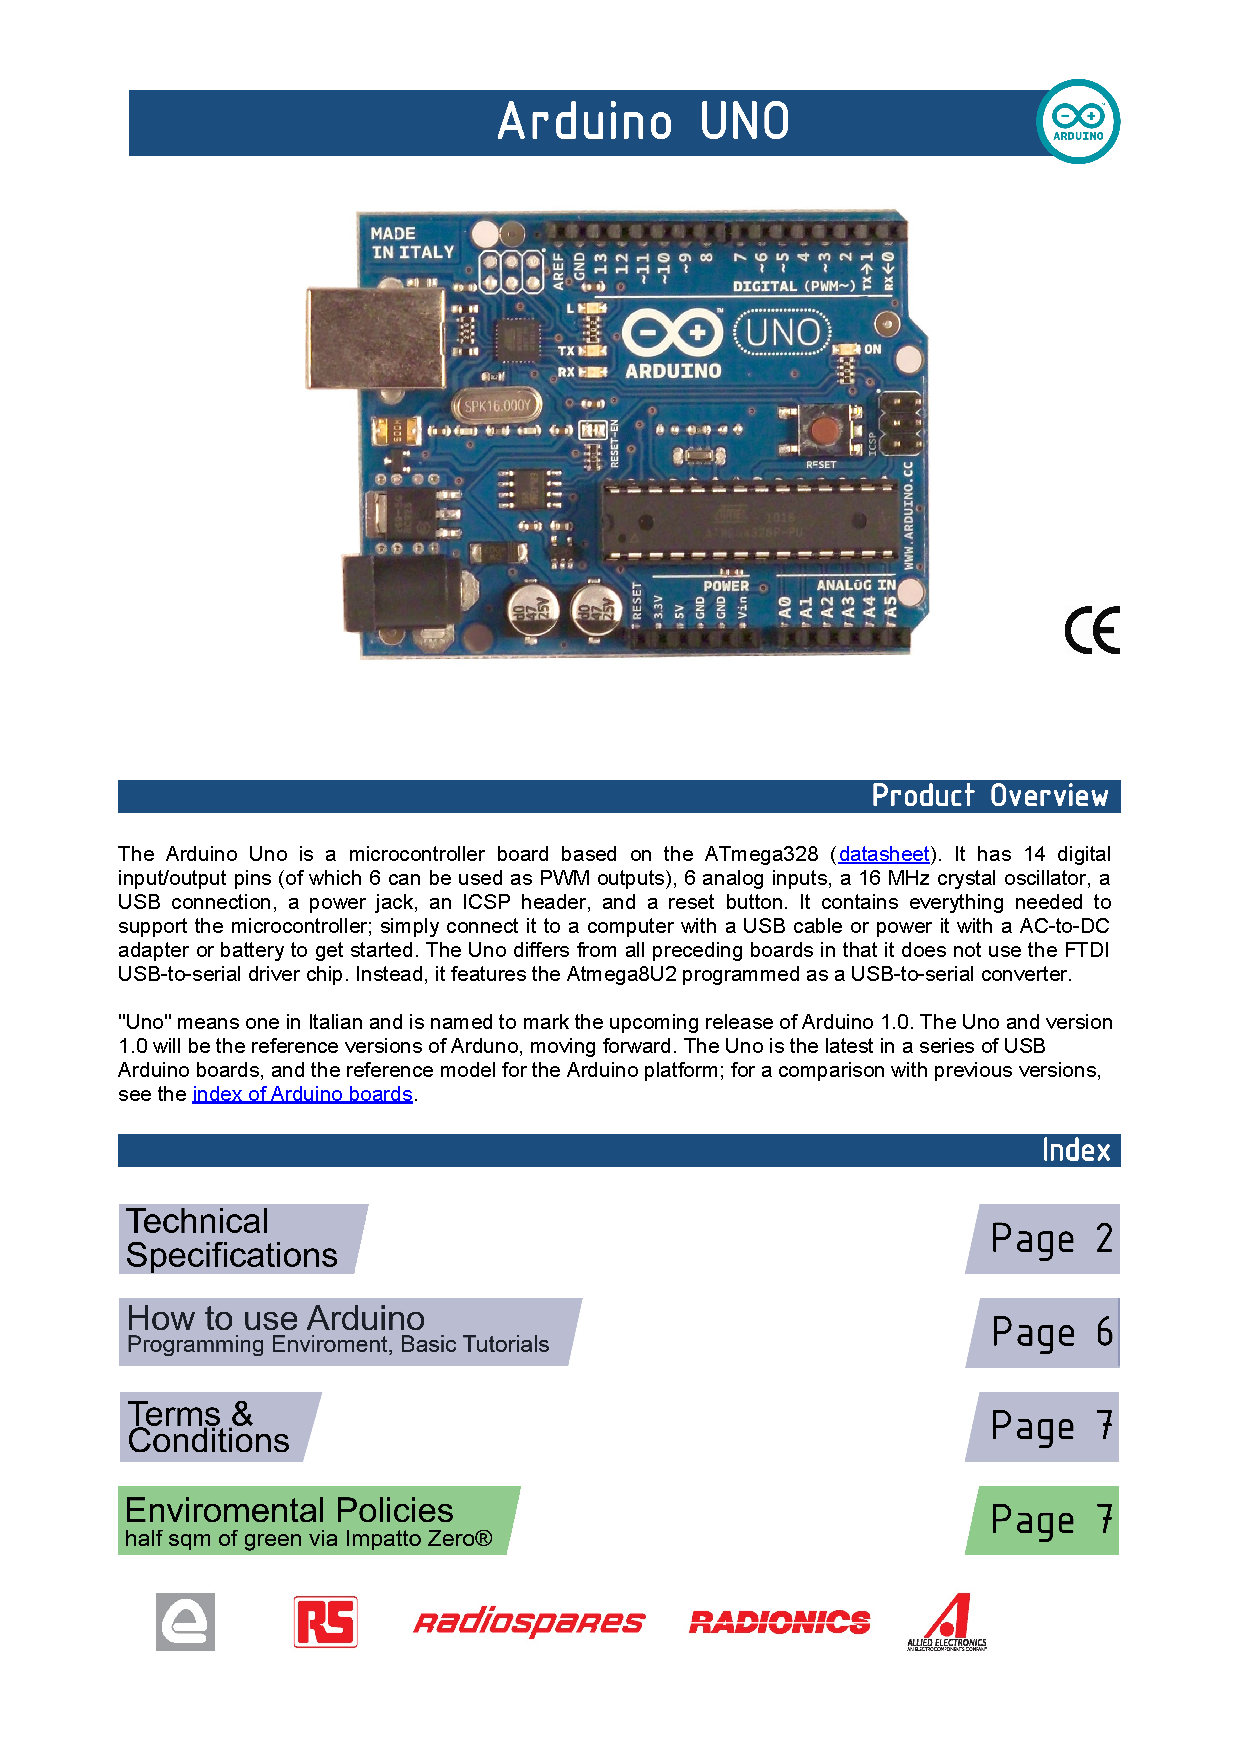
\includepdf[pages={1-2}]{Resources/ARDUINO-UNO.pdf}

\setboolean{@twoside}{true}
\cleardoublepage
\setboolean{@twoside}{false}

\fi
\chapter{Especifica��o t�cnica HC-05}
\label{Anexo}

\begin{figure}[H]
	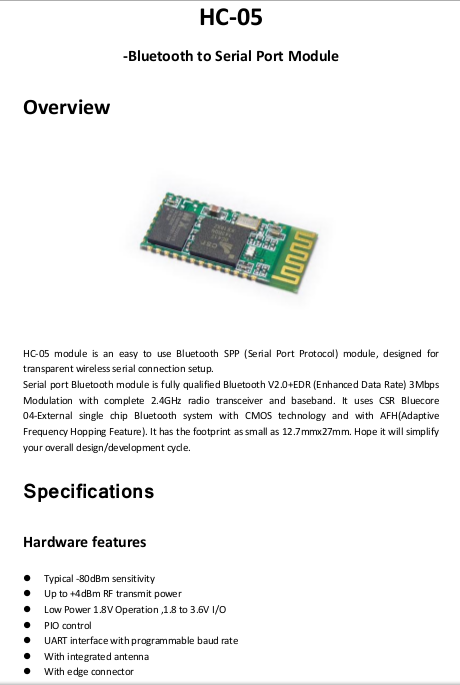
\includegraphics[scale=0.9]{./Resources/hcpageOne.png}
\end{figure}

\begin{figure}[H]
	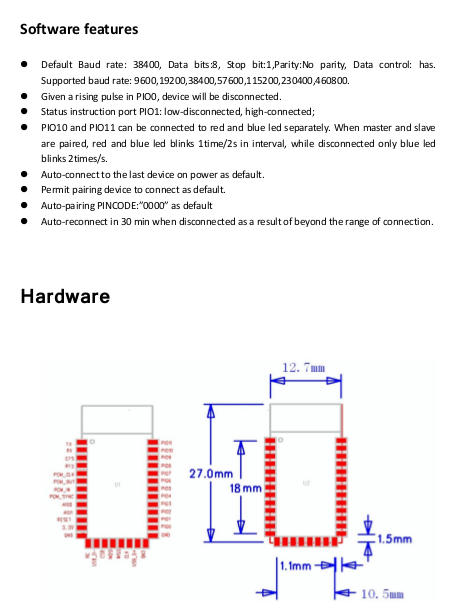
\includegraphics[scale=0.9]{./Resources/hcpageTwo.png}
\end{figure}

%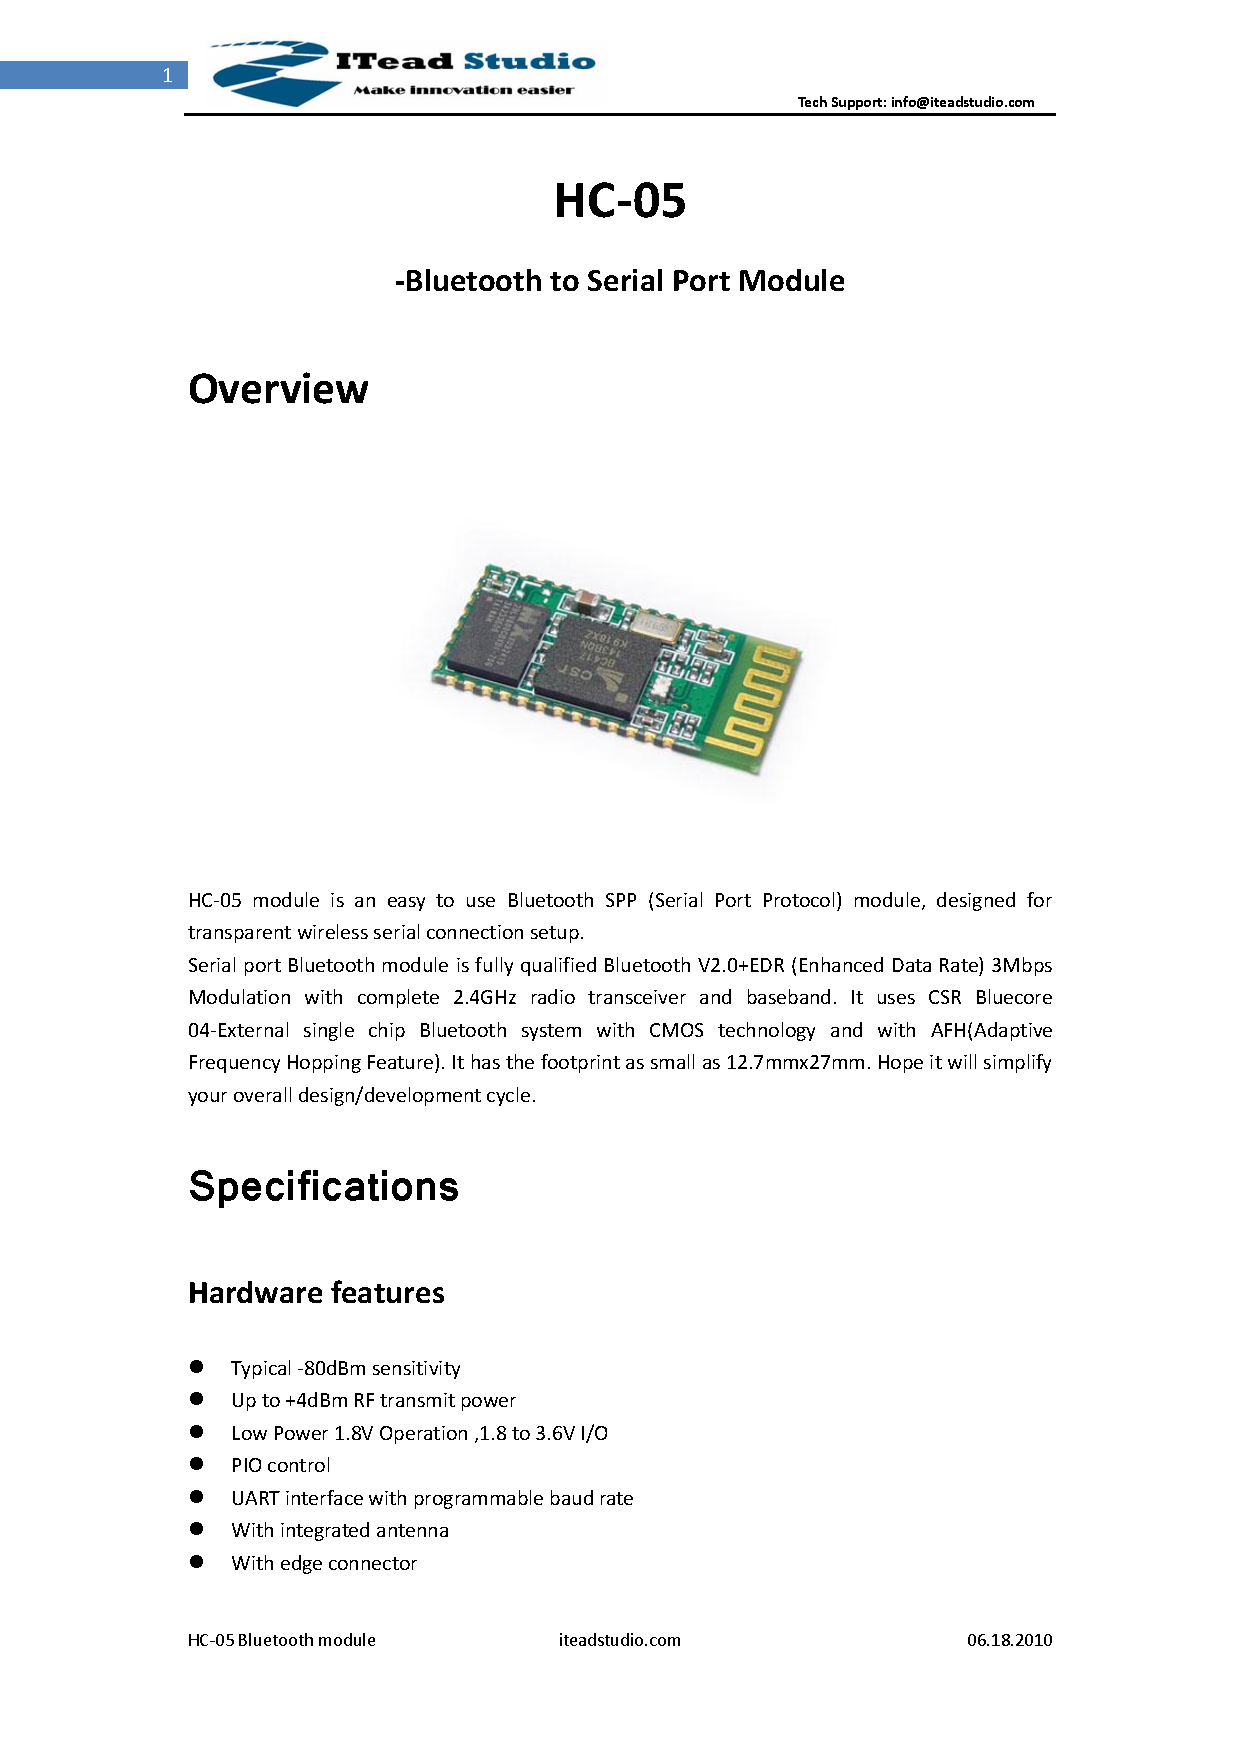
\includepdf[pages=1,pagecommand={\chapter{Datasheet HC-05} \thispagestyle{empty}}, offset=0cm -6cm fitpaper=true]{Resources/HC-05.pdf}

%\includepdf[pages=2,pagecommand={\thispagestyle{empty}}, fitpaper=true]{Resources/HC-05.pdf}

\iffalse
\includepdf[pages={2}]{Resources/HC-05.pdf}


\setboolean{@twoside}{true}
\cleardoublepage
\setboolean{@twoside}{false}
\fi

\chapter{Especifica��o t�cnica HC-SR04}
\label{SensorAnexo}

\begin{figure}[H]
	
\includegraphics[scale=1]{./Resources/hcsrpageOne.png}
\end{figure}

\includepdf[pages={2,3}]{Resources/HCSR04.pdf}